\documentclass[journal,compsoc]{IEEEtran}
\usepackage[nocompress]{cite}
\usepackage[font=normalsize,labelfont=sf,textfont=sf]{subfig}
\usepackage{graphicx}
\usepackage{arabtex}
%\usepackage{fixltx2e}
%\usepackage{stfloats}
%\usepackage{url}
\usepackage[cmex10]{amsmath}
%\usepackage{array}
%\usepackage{mdwmath}
%\usepackage{mdwtab}
%\usepackage{eqparbox}

%packages that were not copied from the IEEE template - need to check if it is valid to add them
\usepackage{amssymb}
\usepackage{multicol}
\usepackage[linesnumbered]{algorithm2e}
\usepackage{color}
\usepackage{etoolbox}
\newtoggle{long-version}
\togglefalse{long-version} 

%TODO: Add biography and image for me and for DR. Raid.
%TODO: Check for plagiarism in all the document.

\begin{document}

\title{Ongoing Segmentation of On-line Handwritten Arabic Script}
%% or ongoing.

\author{George~Kour,
		Raid~Saabne}

%\markboth{Journal of \LaTeX\ Class Files,~Vol.~6, No.~1, January~2007}%
%{Shell \MakeLowercase{\textit{et al.}}: Bare Demo of IEEEtran.cls for Computer Society Journals}

\markboth{\today}{}

%\IEEEspecialpapernotice{(Invited Paper)}


\IEEEcompsoctitleabstractindextext{
\begin{abstract}
the cursive and unconstrained nature of the Arabic script, in both printed and handwritten forms, anneals the task of segmentation. 
While real-time performance is required in applications involving on-line handwriting recognition, most techniques for handwriting recognition wait until the entire curve is traced out before starting the analysis, inevitably causing delays in the recognition process. 
This paper proposes a novel ongoing recognition-based segmentation technique of the on-line Arabic script by carrying out the most time consuming recognition process while the stroke being scribed. 
The system has been designed and tested using the ADAB Database and promising results were obtained.
\end{abstract}
\begin{IEEEkeywords}
Arabic Script Segmentation, Strokes Segmentation, On-line Text Recognition
\end{IEEEkeywords}
}
\maketitle

\IEEEdisplaynotcompsoctitleabstractindextext

\section{Introduction}
\date
\IEEEPARstart{H}{andwriting} remains the most used mean of communication and recording of information in the daily life. 
Therefore, a growing interest in the handwriting character recognition field has taken place in recent years. 
Handwriting recognition can be categorized into two main fields: off-line and on-line. 
In the off-line, a digital image containing text is fed to the computer and the system attempts to convert the spatial representation of the letters into digital symbols \cite{al2011online}. 
On the contrary, in the on-line handwriting recognition, the process is done on a digital representation of the text written on a special digitizer, PDA, tablet or smart-phone device where sensors picks up the pen-tip movements.\\
 
Techniques for cursive text recognition can be split into two main approaches. 
The holistic approach considers the global properties of the written text and recognizes the input word shape as a whole \cite{biadsy2011segmentation, saabni2009hierarchical}. 
The analytic approach involves segmentation and classification of each part of the text \cite{abdulla2008off, sari2002off, Dinges2011}. 
The holistic approach requires the classifier to be trained over the entire dictionary. 
While this is possible for small vocabulary of words, it is impractical for large dictionaries containing 20,000 words or more. 
Under these circumstances, recognizing words using the analytic approach seems to be more feasible \cite{elanwar2012unconstrained}.\\

The cursiveness of the Arabic script, prima facie, requires delaying the launch of the recognition process until the entire word is scribed. 
However, revising this observation one may notice that in most cases significant acceleration of the recognition process can be achieved by approximating the position of the segmentation points while the stroke is being written.\\

In Section \ref{sec:related_work} we mention related studies done in the field of on-line Arabic recognition. 
The proposed approach is described in details in Section \ref{sec:approach} and results are shown in the section \ref{sec:results}. 

\section{Related Work}
\label{sec:related_work}

Randa et al. \cite{elanwar2012unconstrained} have proposed a two stage on-line Arabic handwritten text segmentation system based on Hidden Markov Model (HMM). 
In the first stage, segmentation points were nominated and in the second stage these points were validated using a rules-based engine. 
The system was tested using a self-collected database named OHASD.\\

Laslo Digness et al. \cite{Dinges2011} used a segmentation-based recognition approach based on dividing the word to smaller pieces which afterwards segmented into candidate letters and then classified into letter classes using statistical and structural features. 
$k$-NN classifier was used to obtain the final recognition.\\

A segmentation-based recognition method that operates on the stroke level for on-line Arabic handwritten words recognition was proposed by Khaled Daifallah et al. \cite{daifallah2009recognition}. 
Segmentation points were nominated and then selected by locating semi-horizontal lines moving from right to left. 
A portion of the segmentation points is filtered out by applying on a certain set of rules. 
Then, HMM is used to classify the sub-strokes to letters using Hu feature. 
The candidate and its scoring letters results were used to determine the best set of segmentation points.\\


\section{Approach}
\label{sec:approach}

\textbf{Complexity Measure:} Given a trajectory $S=\{{p_i}\}_{i=1}^{n}$, this value indicates the degree of the trajectory's curvature. 
Preprocessing steps which includes simplification and re-sampling is required to ensure invariance under scaling and disregard the data imperfections. 
The calculation of this parameter is done as follows: for each inner point $p_i$ the parameter $\alpha_{i}$ is computed by:
\begin{equation}
 \alpha_{i}=\frac{\pi-\phi_{i}}{\frac{\pi}{6}}
\end{equation}
where $\phi=\angle(\overline{p_{i-1}p_{i}},\overline{p_{i}p_{i+1}})$.\\ 
The complexity measure is then defined as:
\begin{equation}
CM(S)=\Sigma_{i}\alpha_{i}
\end{equation}\\

%{\color{blue}
%Below, a digest of the main stages of our approach (see Figure \ref{fig:system_flow}):\\
%\textbf{Stage 1.}  \emph{Points of interest} (POIs) are identified as potential segmentation points which are continuously nominated while the stroke is being scribed. The sub-strokes imposed by these POIs are scored by a Arabic letter classifier.\\
%\textbf{Stage 2.} Once the entire stroke is available, a rules-based process is used to refine the POIs and re-score the sub-strokes.\\
%\textbf{Stage 3.} The system heuristically determines the final set of segmentation points based on the sub-strokes scoring.}\\

\begin{figure}
\centering
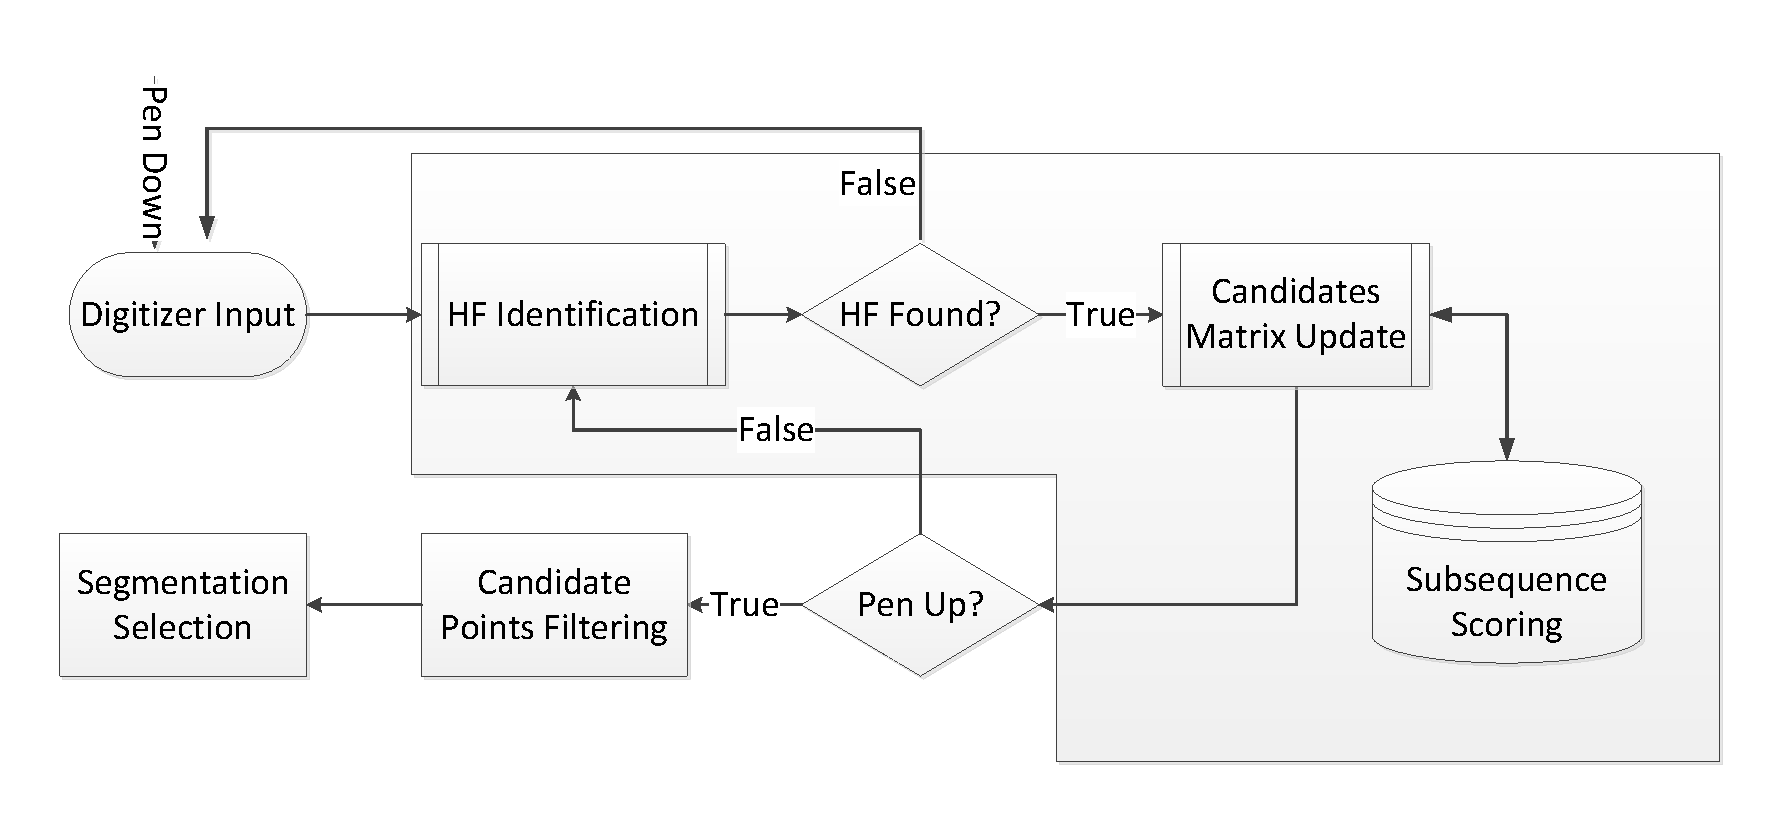
\includegraphics[width=1.05\columnwidth]{./figures/system_flow}
\caption{High level system flow. The first stage is multi-phase and contain three subcomponent. }
\label{fig:system_flow}
\end{figure}

\subsection{First Stage: nomination of POIs and sub-strokes scoring}

\textbf{Horizontal Fragment identification:} in this stage the system attempts to identify \emph{horizontal fragments} (HFs) which join pairs of connected letters. 
These handlers are horizontal, directed right to left and located near the baseline (see Figure  \ref{fig:horizontal_fragments}). 
Using a smoothed version of the trajectory helps the process to ignores undesired small horizontal regions that are frequently caused by the digitizer imperfection.  
A point $p_{i}$ is defined as a "horizontal point" if the slope of the line $\overline{p_{i-1}p_{i}}$ is less than a threshold value $\delta$. T
his value was empirically tuned to $0.6$. 
The same exact value for this parameter was found independently in \cite{daifallah2009recognition}.\\

\begin{figure}
\centering
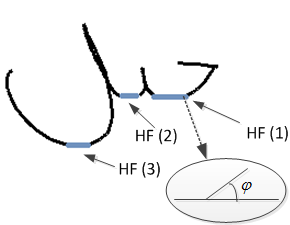
\includegraphics[width=0.5\columnwidth]{./figures/horizontal_fragments}
\caption{Horizontal Fragments [HF] of the word \RL{jbl}(JABAL)}
\label{fig:horizontal_fragments}
\end{figure}

HFs are continuously identified using the following process: 
The first detected horizontal point is set as a "HF starting point". 
All the subsequent horizontal points are ignored until a non horizontal point is obtained indicating the end of HF sequence. 
This point is identified as a "HF ending point" and the medial point of an HF is marked as \emph{point of interest} (POI). 
POI are potential segmentation points and thus this process result in an over-segmentation of the stroke. 
While false positive segmentation points can be easily removed, missed real segmentation points cannot be easily recovered. 
Therefore, in order minimize the miss rate, this process is delicate and allows false HFs to be detected.\\

In a post processing step, fractions of the same horizontal segment identified as multiple HFs are rejoined to a single HF. 
The merging is done by evaluating the complexity measurement across the two consequent HFs, see Figure \ref{fig:candidate_in_no_horizontal}.\\

\begin{figure}
\centering
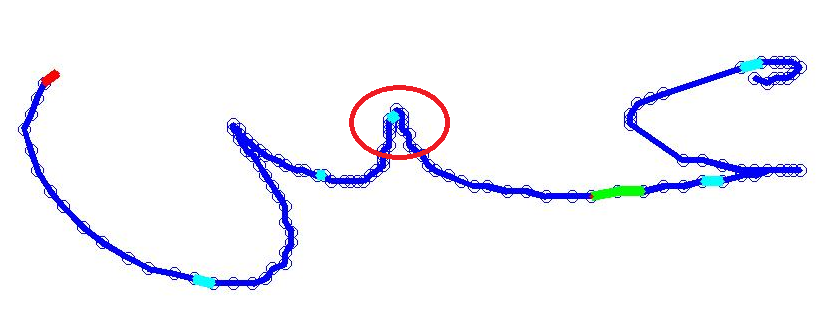
\includegraphics[width=0.5\columnwidth]{./figures/candidate_in_no_horizontal}
\caption{The main body of Arabic word \RL{`yn}. POIs are colored in cyan. The green areas ensigns that HFs merge has taken place. Three types of false POIs can be seen: 1. A POI at the beginning of a stroke. 2. A candidate point that do not reside on a HF. 3. A POI on the valley of the letter \RL{-n}. }
\label{fig:candidate_in_no_horizontal}
\end{figure}

\textbf{Sub-stroke Scoring:}
Let $S=\{p_{i}\}_{i=1}^{n}$ be a 2-D sequence representing a handwritten stroke in which $L$ POIs were detected. 
Let $KP=\{KP_{i}\}_{i=0}^{L+1}$ (Key Points) a set containing the identified POIs in addition to the first and the last points of the stroke as the first and the last items of the set.
Formally, we define: 
\begin{equation}
KP_{i} =\begin{cases}    1		, & \mbox{if } i=0 \\
							   POI_{i}	, & \mbox{if } 1\leq i \leq L \\
							   n    , & \mbox{if } i=L+1 
			\end{cases}				
\end{equation}

A sub-stroke $S_{i}^{j}$ is a sub-sequence of the stroke $S$ that starts at $KP_{i}$ and ends at $KP_{j}$, formally:
\begin{equation}
S_{i}^{j}=\{p_{k}\}_{k=KP_{i}}^{KP_{j}}; i<j
\end{equation}
We generate an upper triangular scoring matrix $D\in\mathbb{R}^{(L+1)\times (L+1)}$ where each cell $D_{i,j}$ defines the scoring obtained by the classifier for the sub-strokes in $S_i^j$. 
The matrix $D$ is generated dynamically adding a row and a column for each new detected POI. 
A locality constraint which narrows the band of the $D$ matrix above the main diagonal improves efficiency and segmentation accuracy. Given a band width $B$ we fix:
\begin{equation}
D_{i,j}=\infty \Leftrightarrow j \leq i \vee j-i>B 
\end{equation}
Scores of sub-strokes representing a letter will achieve, in most cases, better resemblance scoring, i.e., $D_{i,j}$ value will be relatively smaller than for other sub-strokes.\\

\begin{figure}
\centering
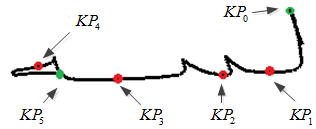
\includegraphics[width=0.7\columnwidth]{./figures/candidate_points}
\caption{Key Points of the word \RL{lbyh}. The first and last key points are colored in green. The red points are the candidate points}
\label{fig:candidate_points}
\end{figure}

The scoring system contains four databases, one for each letter position. It receive a sequence and a position (Ini, Mid, Fin and Iso). A stroke may represent an entire or a fraction of a WP or a portion of a WP that contain the following letter positions: 
\begin{multicols}{2}
\begin{itemize}
    \item $Iso$
    \item $Ini,Mid^{*}$
    \item $Mid^{+}$    
    \item $Mid^{*},Fin$
    \item $Ini,Mid^{*},Fin$
\end{itemize}
\end{multicols}
where $^{+}$ represents one or more occurrences and $^{*}$ represents zero or more occurrences.\\

In order to reduce the number of databases to be searched in, we define four types of subsequences. Given the stroke $S$ containing $L$ POIs we define: 
\begin{itemize}
	\item \textbf{$\alpha$ subsequence:}  A sub-sequence $S_0^k$ where $ 1\leq k < L+1$. It may contain an initial or medial letter only.
	\item \textbf{$\beta$ subsequence:}  A sub-sequence $S_m^k$ where $m \geq 1 \wedge m< k \leq L$. It may contain a medial letter only.
	\item \textbf{$\chi$ subsequence:}  A sub-sequence $S_m^{L+1}$ where $m \geq 1$. It can contain only a medial or final letter.
	\item \textbf{$\delta$ subsequence:} A sub-sequence $S_0^{L+1}$. It can represent letter in any position.
\end{itemize}

The type of the database to be examined for a given cell in $D$ is indicated in the corresponding cell in the matrix $D_p$ (see Matrix in Equation \ref{eq:positions_matrix}). 

\begin{equation}
D_{p}=
\left( 
\begin{array}{ccccccc}
\infty 	& \alpha & \alpha & \alpha  & \cdots & \alpha & \delta \\
\infty  & \infty  & \beta   & \beta   & \cdots  & \beta  & \chi    \\
\infty  & \infty  & \infty   & \beta   & \cdots  & \beta  & \chi    \\
\vdots & \vdots & \vdots  & \vdots & \ddots  & \vdots & \vdots \\
\infty  & \infty  & \infty   & \infty   & \cdots  & \beta  & \chi    \\
\infty  & \infty  & \infty   & \infty   & \cdots  & \infty  & \chi    \\
\infty  & \infty  & \infty   & \infty   & \cdots  & \infty  & \infty \end{array} \right)
\label{eq:positions_matrix}
\end{equation}

For each subsequence, the recognition system returns the $K$ minimal scored potential different letters (we set $K=3$), see Figure \ref{table:substrokes_demo}.\\


\begin{figure}
\centering
\renewcommand{\arraystretch}{2}
\begin{tabular}{| c |c | c | c| c | c | c |}
\hline
 $KP_i$ & $0$ & $1$ & $2$ & $3$ & $4$ & $5$\\ 
\hline
$0$
   & N/A
   & \subfloat{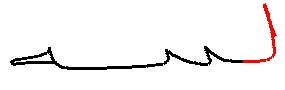
\includegraphics[width=0.8cm]{./figures/substrokes/L}}
   & \subfloat{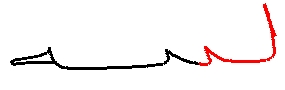
\includegraphics[width=0.8cm]{./figures/substrokes/LB1}}
   & \subfloat{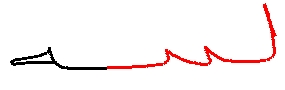
\includegraphics[width=0.8cm]{./figures/substrokes/LB1B2}}
   & N/A & N/A \\
\hline
$1$
   & N/A & N/A
   & \subfloat{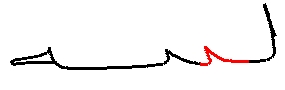
\includegraphics[width=0.8cm]{./figures/substrokes/B1}}
   & \subfloat{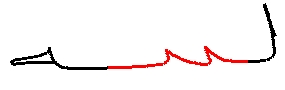
\includegraphics[width=0.8cm]{./figures/substrokes/B1B2}}
   & \subfloat{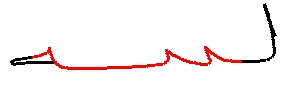
\includegraphics[width=0.8cm]{./figures/substrokes/B1B2H1}}
   & N/A \\
\hline
$2$
   & N/A  & N/A & N/A
   & \subfloat{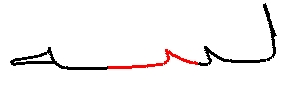
\includegraphics[width=0.8cm]{./figures/substrokes/B2}}
   & \subfloat{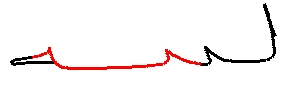
\includegraphics[width=0.8cm]{./figures/substrokes/B2H1}}
   & \subfloat{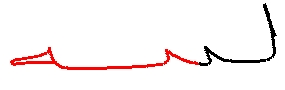
\includegraphics[width=0.8cm]{./figures/substrokes/B2H}} \\
\hline
$3$
   & N/A & N/A & N/A & N/A
   & \subfloat{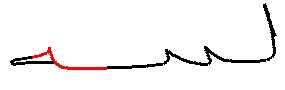
\includegraphics[width=0.8cm]{./figures/substrokes/H1}}
   & \subfloat{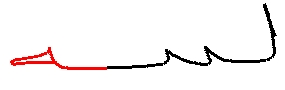
\includegraphics[width=0.8cm]{./figures/substrokes/H}} \\
\hline
$4$
   & N/A & N/A & N/A & N/A & N/A
   & \subfloat{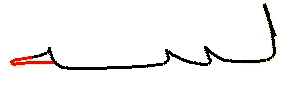
\includegraphics[width=0.8cm]{./figures/substrokes/H2}}\\
\hline
$5$
   & N/A & N/A & N/A & N/A & N/A & N/A \\
\hline
\end{tabular}
\caption{Visual demonstration of subsequences of the word shown in figure \ref{fig:candidate_points}}
\label{table:substrokes_demo}
\end{figure}

\subsection{Second Stage: Candidate points filtering and scoring correction}
In this stage we eliminate redundant segmentation points found in the over-segmentation based on the following rules:

\begin{itemize}
	\item[] \textbf{Rule 1:} Inner Segmentation point lies close to the baseline. 
	\item[] \textbf{Rule 2:} Segmentation points do not reside in loops.
	\item[] \textbf{Rule 3:} A sub-stroke length is proportional to the length of the containing stroke.
\end{itemize}

In order to detect whether a POI is a possible segmentation point we consider its distance to the stroke baseline. Inaccurate baseline position is not critical in our case because we need only to make sure that the candidate points are in a reasonable distance from the baseline. POIs located inside loops are filtered out. The calculated ratio of the sub-stroke length/ containing stroke width is used to penalize POIs with very low ratios. To figure the threshold for filtering we use the anticipated number of letters derived from the number of POIs. We use the third rule is to avoid high scoring resulted for discordant scaling of the letters. To illustrate the discordant scaling problem, see figure below. The suffix of the letter \RL{d} is very similar to the letter \RL{-a}. The only way to visually discriminate between them is by comparing the scaling of this suffix to the whole stroke dimensions.

In some cases candidate segmentation points are incorrectly nominated on areas that are not horizontal, this is caused from the fact that the nomination is done while the word is being scribed, and our filtering algorithm should be corrected to handle this case.

In several cases we encountered POIs that reside on the same horizontal fragment. This may result from scaling problems and also  . We filter out this redundant candidate points in the nomination process and do not wait till this filtering phase. The reason is that since we calculate a narrow band of the Scoring matrix, leaving the impermissible candidate points will result in low performance since highly over segment the word will cause also the system to miss letters because we calculate only a portion a narrow band of the scoring matrix. If such case is identified by the nomination algorithm the medial point between the adjacent candidate points is taken.

\textbf{Baseline detection:} The baseline is determined by calculating the vertical density histogram of the re-sampled sub-stroke. The y-axis is partitioned into $10$ intervals, then, the center of the of the most common interval is calculated $I_{max}$. A $POI$ is filtered out if the following holds:
\begin{equation}
|POI_y-I_{max}|>2*max{({|I|},0.15)} 
\end{equation}
where $POI_y$ represents the $y$ coordinate of the $POI$ and $|I|$ is the length of the interval. In order to reliably determine the baseline, the algorithm is activated only from the fourth POI. This process has proven to be very effective in eliminating challenging false POIs that reside on valleys of frequently used Arabic letters, such as \RL{q}, \RL{s} and \RL{n}, in the their final form. An example of such POI can be seen in the letter \RL{-n} in Figure \ref{fig:candidate_in_no_horizontal}. 

\subsection{Third Stage: Segmentation Selection}
The goal of this phase is to select the best segmentation points set among the POIs. It is done by finding a \emph{segmentation path} in $D$ with the best scoring possible under a preset constraint. A segmentation path $\pi$ is an ordered sub-set of the scoring matrix $D$ cells which has the following form: 
\begin{equation}
\pi=\{\pi_i\}_{i=1}^{i=L}=(1,a_{1}),(a_{1},a_{2}),...,(a_{L-1},a_{L}),(a_{L},n)
\end{equation}
Note that a segmentation path defines a unique the \emph{Final Segmentation Points} ($FSP$).\\

The scoring of the segmentation path $\pi$ is defined as follows:
\begin{equation}
\Pi = \Sigma_{i=1}^{L}{D(\pi_{i})}
\end{equation}

The scoring matrix $D$ can be modeled as a directed weighted edges graph $G=(V,E)$ where a possible segmentation defines a path from vertex $KP_1$ to vertex $KP_{L+1}$. However, in this case, the optimal segmentation is not necessarily obtained by finding the shortest path in $G$. In most cases, greedily selecting the outgoing edge with the minimal value obtains a better segmentation than the one defined by the shortest path.


Several \emph{segmentation selection algorithms} (SSAs) are proposed in this work for finding the best segmentation path, i.e. which represent the correct segmentation of the stroke $S$.

Here we describe two algorithm that were given the names \emph{Forward Segmentation Selection} (FSS) and \emph{Backward Segmentation Selection} (BSS) which are and operate pretty similarly. A pseudo-code of FSS can be seen in Algorithm \ref{alg:fss} below. FSS starts with the first point and advancing toward the end of the stroke. In Each step it tries to find the next best segmentation point by selecting the subsequence $S_i^j$ having the best scoring value (as can be seen in line 5). BSS starts from the last point and advances toward the beginning of the stroke. The drawback of the these two algorithms is that FSS tends to under-segment the suffix of the stroke and BSS tends to under-segment the prefix of the stroke.   

\begin{algorithm}
$i=0$\;
$sum=0$\;
$FSP = \emptyset $\;
\While{$i<L+1$}
{
	$j = \mathop {\arg \min }\limits_k \left( {D\left( {i,k} \right)} \right)$\;
	$FSP = FSP \cup \left\{ j \right\}$\;
	$sum = sum + D\left( {i,j} \right)$\;
	$i=j$\;
}
\caption{Forward Segmentation Selection (FSS)}
\label{alg:fss}
\end{algorithm}

To overcome the aforementioned drawback a third SSA was proposed and was given the name \emph{Backward-Forward Segmentation Selection} (BFSS). As described in Algorithm \ref{alg:bfss}, it combines both FSS and BSS. BFSS operates from the sides of the stroke toward the center. In every iteration the algorithm selects two candidate points to include to the $FSP$. \\

\begin{algorithm}
$poi_{a}=1$\;
$poi_{b}=n$\;
\While{$poi_{a}<poi_{b}$}
{
	$poi_{a,next} = \mathop {\arg \min}\limits_k (D(poi_a,k))$\;
	$FSP = FSP \cup \{poi_{a,next}\}$\;
	$poi_{a}=poi_{a,next}$\;
	
	$poi_{b,next} = \mathop {\arg \min}\limits_k (D(k,poi_{b,next}))$\;
	$FSP = FPS \cup \{poi_{b,next}\}$\;	
	$poi_{b}=poi_{b,next}$\;
}
\caption{Backward-Forward Segmentation Selection (BFSS).}
\label{alg:bfss}
\end{algorithm}
  
The last SSA, that was given the name \emph{Greedy Segmentation Selection} (GSS), operates completely in a different way. In every iteration, the cell with the best scoring is selected. If cell $D(i,j)$ is selected, both the candidate point $POI_{i}$ and $POI_{j}$ are added to FSP and every segmentation point between $i$ and $j$ are removed from the scoring matrix by setting to $\infty$ in the corresponding cells in $D$. This, to avoid those candidate point to be selected in a later iteration. 

\begin{algorithm}
$FP=\emptyset$\;
\While{$CPS \neq \emptyset$}
{
	${s,e} = \mathop {\arg \min}(D)$\;
	$FSP = FSP \cup \{s,e\}$\;
	$sum = sum + D(s,e)$\;
	$UpdateMatrix(D,s,e)$\;
	$CPS = CPS\setminus\{s,e\}$\;
}
$FP=FP\setminus\{1,n\}$\;

\caption{Greedy Segmentation Selection (GSS)}
\label{alg:gss}
\end{algorithm}

FSS, BSS, BFSS and GSS are executed independently for each stroke. The $FSP$ with the smallest $\Pi$ is selected. Evaluations of the mentioned SSA is provided in \ref{subsec:ssa_performance}. 



\section{The ADAB Database}
\label{sec:database}
The ADAB database is de-facto a standard in the on-line Arabic handwriting recognition field. It is freely available and consists of more than 20k Arabic handwritten words (city names in Morocco) scribed by more than 170 different writers. 
In figure \ref{fig:sample_parts} we show the parts of a sample.
Unfortunately, the ADAB only provides the data of the strokes for a given city name. 
No information indicating the letters boundaries or WP is provided, thus, extra work was needed to add this information to the database so that it could be used as a letters samples source and as ground truth for the segmentation points.
To provide this additional information, we have employed the skills of a human expert to segment the strokes into letters and determine the words and the WPs bounderies that each sample contain. 
This additional information was saved in an xml file. Delayed strokes are not included in the processed information since it is not considered in the segmentation process.
We have manually segmented more than 15k samples which contains about 40k strokes. 

\begin{figure}
\centering
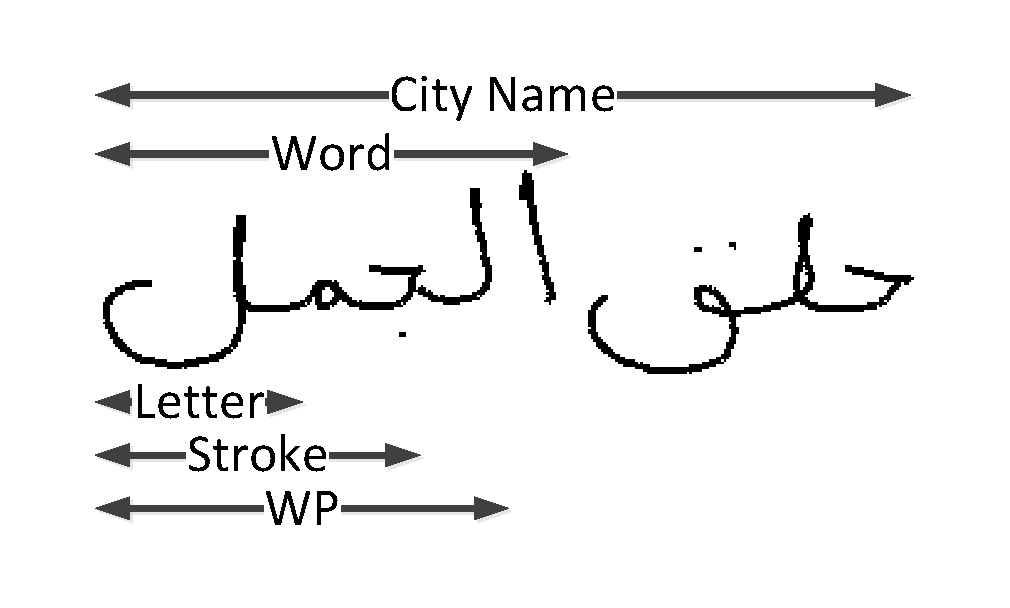
\includegraphics[width=0.3\textwidth]{./figures/sample_parts}
\caption{Visual demonstration of a test sample parts.}
\label{fig:sample_parts}
\end{figure}

\section{Validation}
\label{sec:validation}
Other researches in this area usually use a human expert to validate the accuracy of the segmentation points. However, in this work, we applied an automatic validation process using the ground truth information provided by the database. We discriminate between three types of final segmentation point. A final segmentation point is classified as true positive if the complexity measure between the identified point and a true segmentation point is less than a preset threshold, otherwise it is is classified as false positive. A miss (i.e, false Negative) is the case when the system failed to identify a segmentation point. Although, this validation process was tested on several sets and found to be highly accurate, it was used only on the validation set.

%A Segmentation point can be considered one of the following: 1. Valid (true positive): the segmentation point is identified in the correct location. 2. Invalid (false positive): the segmentation point was identified in an incorrect place. 3. Missing: No segmentation point was identified between two successive letters.

\section{Experimental Results}
\label{sec:results}
The system is implemented using the Matlab environment. Comparing the performance of our approach to other research done in the field is not a simple task. The complexity of such task is not only the different experimental settings, databases and methodology but also the different parameters that are used to display the work results. For this reason, to make our results clear we have chosen to display them from two points of view. The first is the WP and the second is the segmentation point. For the WP, we measured the Segmentation rate (SR) and the Recognition rate (RR).  The usage of the ADAB database instead of an own collected database give our results further firmness. In table \ref{table:general_stats} we provide basic statistics of our sample set.\\

\begin{table}[h]
\caption{General statistics}
\begin{tabular}{ | c | c | }
  \hline
  Number of test samples (city name) & 319 \\
  \hline
  Number of WPs & 1148 \\
  \hline
  Number of Strokes & 1237 \\
  \hline
\end{tabular}
\centering
\label{table:general_stats} 
\end{table}

The results shown in table \ref{table:wp_results} summarizes the system performance in the WP level and in table \ref{table:sp_results} we provide experimental results in the segmentation points level. 

\begin{table}[h]
\caption{WP Results}
\begin{tabular}{ | c | c | }
  \hline
  Segmentation Rate &  83\% \\ 
 \hline
  Recognition Rate &  78\% \\ 
 \hline
  Average Time & 0.64 [sec] \\
\hline
\end{tabular}
\centering
\label{table:wp_results} 
\end{table}

\begin{figure}
\centering
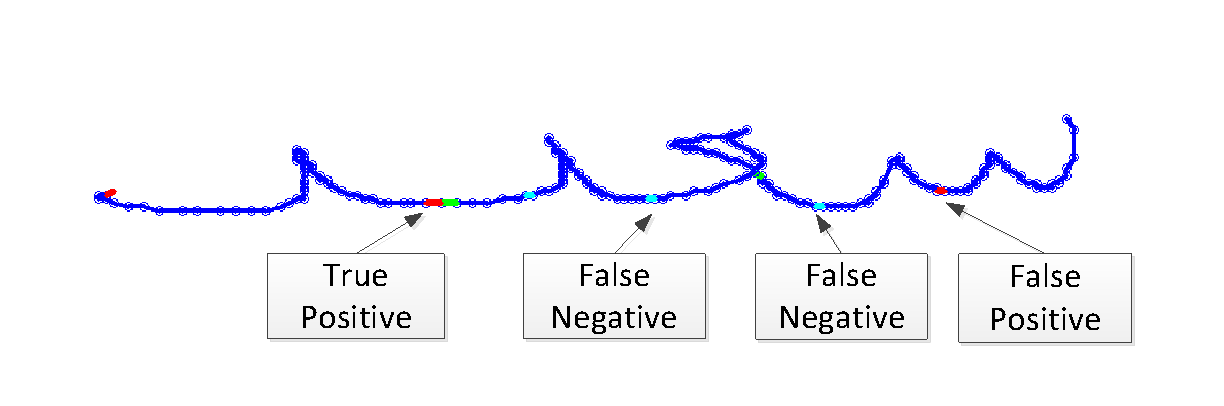
\includegraphics[width=0.9\columnwidth]{./figures/sp_types}
\caption{Segmentation points types.}
\label{fig:sp_types}
\end{figure}

\begin{table}[h]
\caption{Segmentation Points Results}
\begin{tabular}{ | c | c | }
  \hline
  Total number of Segmentation point & 1081 \\
  \hline
  Valid SP (True Positive) & 922 \\
  \hline
  Invalid SP (False Positive) & 119 \\
  \hline
  Missing SP (False Negative) & 159 \\
  \hline                                    
  Precision & 88.6\% \\ 
 \hline
  Recall &  85.3\% \\ 
 \hline
\end{tabular}
\centering
\label{table:sp_results} 
\end{table}

The absolute majority of the false negative segmentation points were identified as POI in the first stage. A small number were filtered out in the filtering phase but most of them were not selected by the SSA.

\subsection{Analysis}
In this section we discuss common cases of incorrect segmentation.
\subsubsection{Over-segmentation}
\textbf{Case 1:} Several Arabic letters contain a horizontal region in their initial form which do not contain a segmentation point but was falsely identified as an HF in the first stage. However, this issue was overcame by adding the following rule: A POI is nominated only if the sub-stroke that spans from the beginning of the stroke to the POI is has a high complexity measure, see Figure \ref{fig:oversegmentation_begin_1}.\\

\textbf{Case 2:} Over segmentation can be caused also from typing a letter in unusual form where it is spanned over several strokes. It happens mostly in the letter forms \RL{-m-}, \RL{-m} (as can be seen in Figure \ref{fig:2_strokes_m}) and in rare cases in the letter \RL{-.h-}.

\begin{figure}
\centering
        \subfloat[]{
           \label{fig:2_strokes_m}
           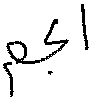
\includegraphics[width=0.16\columnwidth]{./figures/2_strokes_m}
        }
        \qquad
        \qquad
        \subfloat[]{
        	  \label{fig:oversegmentation_begin_1}
           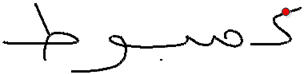
\includegraphics[width=0.6\columnwidth]{./figures/oversegmentation_begin_1}		
        }        
    \caption{An example of writing a single letter using more than a single strokes is shown in \ref{fig:2_strokes_m}. In \ref{fig:letters_same_body} an example of a HF at the beginning of the stroke which do not contain a segmentation point.}
   \label{fig:over_segmentations}
\end{figure}

\subsubsection{Under-segmentation}
\textbf{Case 1:} No HF is identified. mainly results from letter pairs that do not contain horizontal joint between them. This issue is partially solved by extending the notion of a letters to include such pairs. For example the pair \RL{lm} and \RL{l.h}.\\

\textbf{Case 2:} HF is identified but the corresponding POI is not selected in the third stage. This result from a low scoring and thus not being selected by the SSA.\\

In addition, differentiating between the main body of the letter \RL{-s-} and the main body of two consecutive \RL{-b-} letters is impossible without taking into consideration the additional strokes, thus both cases were considered correct.\\

\subsection{Sample set size and distribution}
Since our letters samples are extracted from a real database, the sample set distribution is imbalanced. On the one hand, it can be viewed as an advantage since the letters samples  distribution will reflect the a-priory probability of a letter appearance. On the other hand, a highly imbalanced dataset is known to have negative affect on many classification algorithms.
In the following experiment we measure the affect of both a increasingly large training set and the affect of imbalanced sample set on the system performance.
To do so, we allowed an increasing maximal number of samples per a letter position and measured the segmentation and recognition rates of the system as well as on its time performance. Note that increasing the maximal number of samples per class (letter position) increases the imbalance between the classes. The graph in figure \ref{fig:num_letter_impact} shows that the maximal number of letters does not improve much the segmentation and recognition rates. The graph convergences after 200 samples per letter. It is also evident that there is a point where allowing more samples per class may decrease the accuracy of the system.

\begin{figure}
\centering
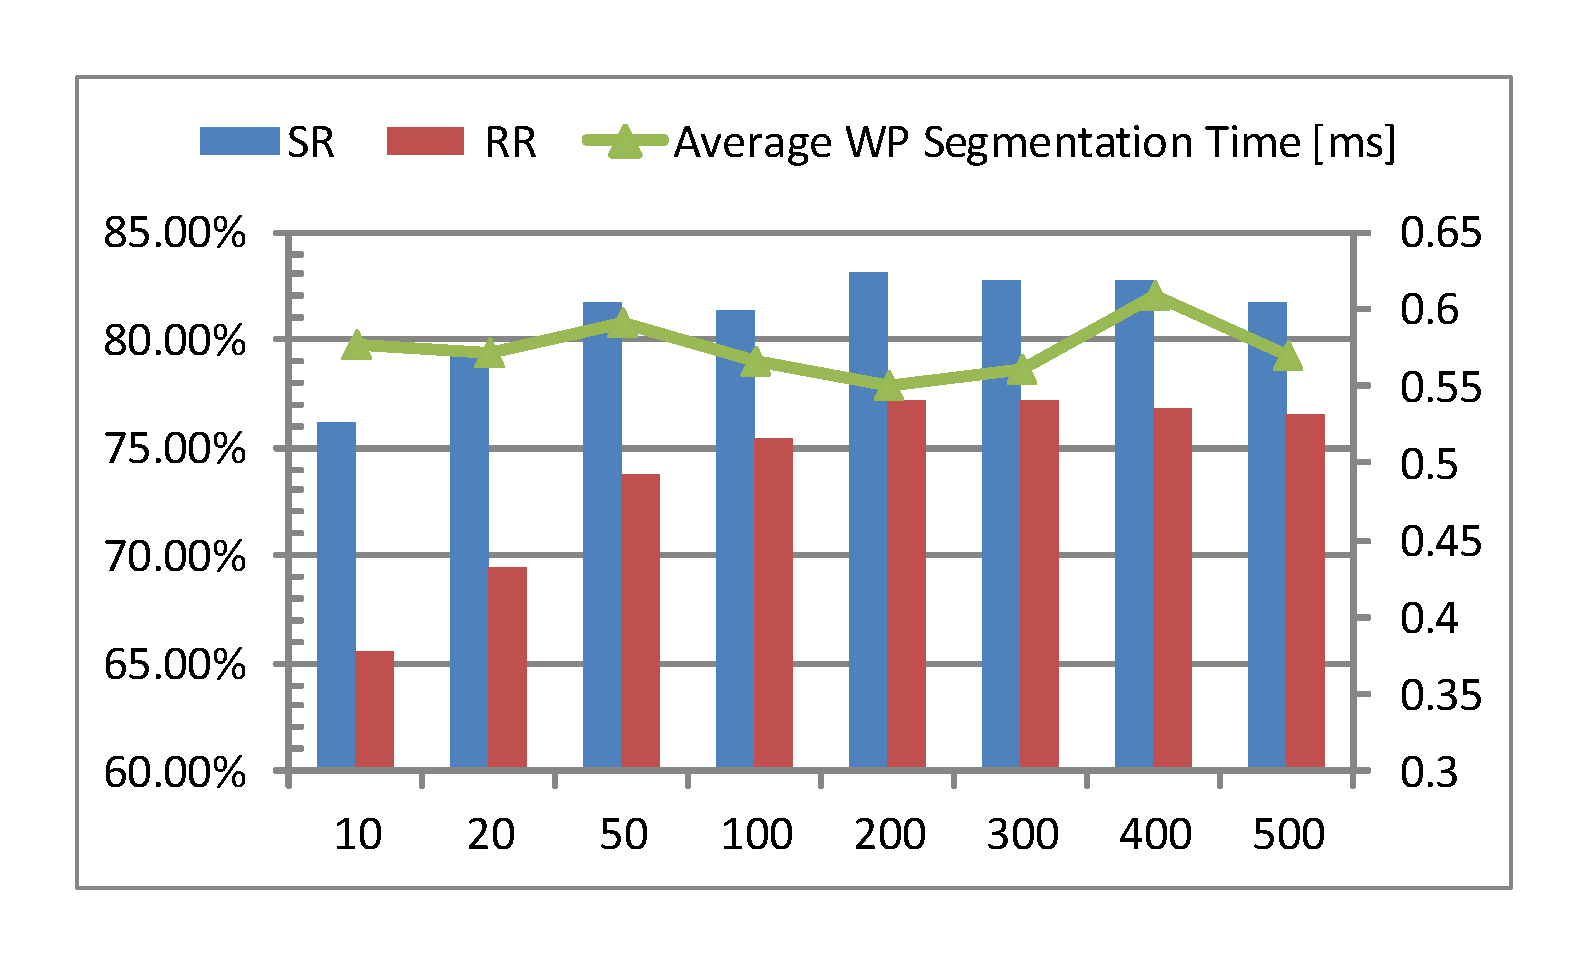
\includegraphics[width=1\columnwidth]{./figures/num_letter_impact}
\caption{The diagram shows the influence of the number of letters samples on the segmentation (SR) , recognition rates (RR) , and the average segmentation time. All the three parameters showing convergence when the maximum letter samples per letter position is larger than 200. }
\label{fig:num_letter_impact}
\end{figure}

\subsection{Segmentation Selection Algorithms performance}
\label{subsec:ssa_performance}
As can be seen in table \ref{table:ss_algorithms_results} the SSA has a crucial affect on the system performance. We tried to combine two SSA by running both SSA and select the segmentation with the smallest scoring divided by the size of $FSP$ to prevent giving superiority to segmentations with less segmentation points. Combination of two algorithms is symboled by $\oplus$.

\begin{table}[h]
\caption{SSA Performance}
\begin{tabular}{ | c | c | c | c | c |}
\hline
SSA & WP SR & WP RR & SP Precision & SP Recall\\
\hline                 
  FSS & 76\% & 70\% & 85\% & 78\% \\ 
  \hline
  BSS & 79\% &  73\% & 84\%& 81\% \\
  \hline
  BFSS & 78\% & 72\% & 84\% & 80\%\\ 
  \hline
  GSS & 80\% & 74\% & 81\% & \bf{94}\% \\  
  \hline
  FSS$\oplus$BSS & \bf{82}\% & \bf{76}\% & \bf{89}\% & 82\%\\  
  \hline
  GSS$\oplus$BFSS & 81\% & 75\% & 83\% & 90\% \\
  \hline
\end{tabular}
\centering
\label{table:ss_algorithms_results} 
\end{table}
\bibliographystyle{IEEEtran}
\bibliography{IEEEabrv,bibliography}

\end{document}


